\documentclass[a4paper, oneside]{memoir}% Document class
\usepackage[a4paper]{geometry}			% Margins
\usepackage{lmodern}
\usepackage{graphicx}
\usepackage{float}
\usepackage{listings}
\usepackage[small,compact]{titlesec}	% No 'chapter' in chapter headings.
\graphicspath{{Media/}}					% Directory that holds images.

\titleformat{\chapter}[hang]
{\normalfont\Large\bfseries}{\thechapter}{1em}{\Large}
\titlespacing{\chapter}{0pt}{*0}{*1}

\titleformat{\chapter}{\Huge\bfseries}{\thechapter}{1em}{}
\titleformat{\section}{\LARGE\bfseries}{\thesection}{1em}{}
\titleformat{\subsection}{\Large\bfseries}{\thesubsection}{1em}{}
\titleformat{\subsubsection}{\normalsize\bfseries}{\thesubsubsection}{1em}{}

\usepackage[draft]{fixme}				% FixMe notes.
\usepackage[disable]{todonotes}					% Todo Notes
\newcommand{\bycykelwithoutspace}{Aalborg Bycykel}
\newcommand{\bycykel}{\bycykelwithoutspace{ }}

\begin{document}
	\thispagestyle{empty} %fjerner sidetal

\hspace*{-1cm}\parbox[b][\textheight][t]{\textwidth}
{

\begin{center}
	
\includegraphics[height=5.2cm]{aau-logo-vector}\\
	\vspace{0.25cm}
	%Student Report
\end{center} 

\vspace{1cm}
\begin{center}

\textbf{\Huge {Software 7 - Bicycles and the Internet of Things}} \\ \vspace{0.5cm}
%\textbf{\Large {Developing Complex Software Systems:}} \\ \vspace{.5cm}
%\textbf{\huge {GIRAF Web Admin and GIRAF Timer}} \\ \vspace{1cm}
\textbf{\Large P7 Project by sw707f14}\\ \vspace{0.5cm}
\textbf{\large 3-9-2014 to 19-12-2014}\\
\end{center}



\vspace{0.25cm}
\begin{center}
\item {\textbf{Participants:}} \\
Dennis Jakobsen\\ Erik Sidelmann Jensen\\ Lasse Vang Gravesen\\ Lars Andersen\\ Mathias Winde Pedersen\\ Søren Skibsted Als\\
\end{center}

\thispagestyle{empty}

\newpage
\thispagestyle{empty}
\mbox{}
}
	\newpage\null\thispagestyle{empty}\newpage
	% Titelbladseksempel til brug på Første studieår.
% Hans Hüttel - hans@cs.aau.dk
% 16. december 2011

% Her begynder selve titelbladet

\thispagestyle{empty}
\begin{titlingpage}
 \begin{nopagebreak}
 {\samepage 
 \begin{tabular}{r}
\parbox{\textwidth}{  \raisebox{-7mm}{
\includegraphics[height=4cm]{aau-logo-vector}}
 \hfill \parbox{4.9cm}{\begin{tabular}{l}
{\small Fourth study year} \\
{\small Software} \\
{\small Selma Lagerlöfsvej 300} \\
 \end{tabular}}
}
% \\
\end{tabular}

 \begin{tabular}{cc}
\parbox{7cm}{
\begin{description}

\item[Title:] 

Software 7 - Internet of Things, Bikes
  
\item[Theme:]

Internet of Things


 \end{description}

\parbox{8cm}{

\begin{description}
\item[Project period:]
    P7, autumn semester 2014 \\
  \hspace{4cm}
\item[Project group:]
	sw707e14 \\
\hspace{4cm}
\item[Participants:] \mbox{} \\[3mm]
Dennis Jakobsen\\ Erik Sidelmann Jensen\\ Lasse Vang Gravesen\\ Lars Andersen\\ Mathias Winde Pedersen\\ Søren Skibsted Als
   \hspace{2cm}
\item[Supervisor:] \mbox{} \\[3mm]
 Hua Lu \\
\end{description}
}
\begin{description}
 \item[Copies:] 8
 \item[Content Pages:] \pagedifference{startoftoc}{lastpagewithoutappendix}
 \item[Appendix:]  \pagedifference{lastpagewithoutappendix}{LastPage}
 \item[Total Pages:] \pageref{LastPage}
 \item[Completed:] 28-5-2014
\end{description}
 \vfill } &
\parbox{7cm}{
  \vspace{.15cm}
  \begin{tabular}{l}
  \textbf{Abstract:}\bigskip \\
  \fbox{
  	\begin{minipage}{6.5cm}
  	\bigskip
  	{\vfill{\small % Motivation
The bicycle share system in Aalborg is generally subpar compared to other similar systems.
To improve it would provide a better experience for the users.

% Problem statement
In other systems, such as the Gobike in Copenhagen uses GPS tracking, routing and other generally useful features. 
To create a website and a supporting system allowing for tracking, booking and other such features would improve the existing system and is attempted.

% Approach
To resolve this we develop a booking and administration website for \bycykelwithoutspace, and software for simulating stations and bicycles. We made a booking solution for the users of the system, and for the administrators we created pages to provide overview of the system on a whole.

% Results
The website ended up having many features supporting the use and administration of the system.
  	\bigskip}}
  	
  	\end{minipage}
	}
   \end{tabular}}
 \end{tabular}
}
\end{nopagebreak}
\end{titlingpage}

% Her slutter selve titelbladet
	\addtocounter{page}{4}
	\newpage\null\thispagestyle{empty}\newpage
	\thispagestyle{empty}
\section*{Foreword}
\noindent This report was made at Aalborg University in the first semester of the Software Candidate study by the group sw707e14. 
The report was made as a part of the P7 project in the period 3-9-2014 to 19-12-2014. 
We discussed the current system with Aalborg Kommune, whose cooperation was helpful. 
The project was supervised by Hua Lu, whose supervision was much appreciated. \\ \\

\noindent
\vspace{5mm}
\parbox[h]{4cm}{Dennis Jakobsen}\hspace{0.5cm} \makebox[7cm]{\hrulefill} \\ \\
\vspace{5mm}
\parbox[h]{4cm}{Erik Sidelmann Jensen}\hspace{0.5cm} \makebox[7cm]{\hrulefill} \\ \\
\vspace{5mm}
\parbox[h]{4cm}{Lasse Vang Gravesen}\hspace{0.5cm} \makebox[7cm]{\hrulefill} \\ \\
\vspace{5mm}
\parbox[h]{4cm}{Lars Andersen}\hspace{0.5cm} \makebox[7cm]{\hrulefill} \\ \\
\vspace{5mm}
\parbox[h]{4cm}{Mathias Winde Pedersen}\hspace{0.5cm} \makebox[7cm]{\hrulefill} \\ \\
\vspace{5mm}
\parbox[h]{4cm}{Søren Skibsted Als}\hspace{0.5cm} \makebox[7cm]{\hrulefill} \\ \\

\newpage
	\newpage\null\thispagestyle{empty}\newpage
	
	\label{startoftoc}
	\begin{KeepFromToc}
		\tableofcontents
		\newpage\null\thispagestyle{empty}\newpage
		\newpage\null\thispagestyle{empty}\newpage
		\todototoc
		\listoftodos
	\end{KeepFromToc}
	\label{endoftoc}
	
	\chapter{Introduction}
	%disposition:
%politisk mål
	%infrastruktur(letbane, CO2, )
	%sundhed archimedesaaaa
	
%aalborg bycyklen
%problemer
	%ingen statistik og umuligt at finde om der er en cykel uden at gå hen til station
	%ingen sikring om at der er en cykel tilstede
	
%vores løsning

In the current time of Danish politics, a heavy focus has been put on better health \citep{misc:nationalemaalhelbred}.
Additionally, a great focus has been placed on climate change, and how to tackle this \citep{misc:klima}.
A part of a solution to this is getting more people to use bicycles for transportation especially in urban areas.
This limits CO2 pollution due to people not driving in cars and increase health of people due to exercising when bicycling.
A way to make people bicycle more are bicycle sharing systems \citep{misc:impactofbikeshare}, which appear in several cities \citep{misc:cibi, misc:bycyklen, misc:AltaBicycleShare, misc:aalborgbycykelMain}.

The bicycle sharing system that we focus on is Aalborg Bycykel.
It is a system where several bicycle stations are placed around the city of Aalborg, and when you need a bicycle, you travel to one of those stations and retrieve a bicycle.
Then when you are finished using the bicycle you deliver it back to one of the stations.
However, some immediate problems are associated with the currently active system.

One of the problems with the system is that bicycles can easily get lost and there is no way to locate missing bicycles, other than user reports.
Additionally, for a user to know if some bicycle is available, he has to walk to stations until he finds an available bicycle.
Furthermore, if a user wants to be more certain that he can retrieve a bicycle in the near future, there is no way to ensure this other than retrieving a bicycle ahead of time.

These are some of the central issues that is sought to be resolved with the developed system described in the following chapters.
In the developed system, we take other existing bicycle sharing systems into account \citep{misc:cibi, misc:bycyklen, misc:AltaBicycleShare}.
On the basis of this, a booking and status system is developed for the users, and a tracking and statistics system is developed for Aalborg Kommune.

Some of the technical challenges we encounter are communication between different parts of the system, which we achieve with SOAP and TCP, how to synchronise state across these different parts, which we address with well considered rules.
Additionally, we discuss how to design the system to reach a good usability standard, where we prioritise simple solutions over advanced solutions and in addition to this utilise usability tests.

The report contains the following chapters:
\begin{itemize}
\item Analysis - The analysis is documented resulting in a problem definition as well as a specification of the requirements and target audience.
\item Suggested Solutions - Solutions to different problems in the problem domain are suggested.
\item Technologies - Different technologies and concepts used for this project are documented.
\item Design - The design of the overall system is documented.
\item Implementation - The implementation of the designed system is documented.
\item Test - Unit and usability tests are documented. 
\item Discussion - Decisions about the overall system and why they were made are documented. The developed system is compared to other existing systems. Additionally, further development is documented.
\item Conclusion - Verifies the hypothesis according to the questions asked in the problem definition.
\end{itemize}
	\chapter{Analysis}
	This chapter includes analysis of the current system already in place in Aalborg, other existing systems, the problem definition, and general requirements.
	\section{Current System}\label{sec:currentsystem}

%Disposition
%kort introduction til hvad det er
%scenarier hvor bycyklen kan bruges
%hvem vedligeholder det
%cyklernes placering
%Positive erfaringer med bycyklen, ref god kilde

\bycykel is a bicycle system where people in Aalborg are able to borrow bicycles to travel around the city.
The system was started in September 2008 as part of the CIVITAS ARCHIMEDES project, which focuses on making bicycles more widely used \citep{misc:aalborgcykling}.
The bicycles can be found in stations located around the city of Aalborg, for exact placement of the bicycles see \figref{fig:CykelLokationer}.
As can be seen, the bicycles are mostly located in the center of Aalborg.

\begin{figure}[h]
	\centering
	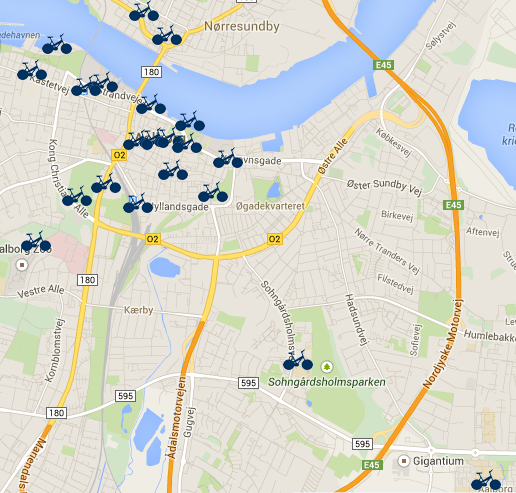
\includegraphics[scale=0.75]{analysis/CykelLokationer}
	\caption{Bicycle locations \citep{misc:aalborgbycykel}.}
	\label{fig:CykelLokationer}
\end{figure}

In 2009, 135 bicycles was placed in Aalborg, and in 2012 this number had been increased to 200 bicycles \citep{misc:aalborgcykling}.
In order to borrow a bicycle, you need to go to one of the bicycle stations, deposit 20 DKK to unlock the bicycle, then return it to a station when you are done with the bicycle, where you then retrieve your 20 DKK, which makes the system free to use \citep{misc:aalborgbycykelregler}.
The system is built on trust, because if people do not return the bicycles to a station when finished using them, the bicycles gradually disappear.

\bycykel has had, as of 2012, success with their system. 
According to a report, if the system had not been in place more than half of the users would have walked and 5 percent would have driven in a car instead \citep{misc:aalborgcykling}.
Furthermore, it shows that over three seasons the percentage of bicycles lost have been at maximum 11\% \citep{misc:aalborgcykling}.

As the bicycles are borrowed by depositing 20 DKK, no consequences exist for not returning the bicycle except for losing the deposit.
This can lead to bicycles getting lost and as there is no additional monitoring of where the bicycles are located around the city, other than travelling around the city to locate the bicycles, which is a problem.
Another problem of not monitoring the position of the bicycles is that it can be difficult for Aalborg Kommune and the potential users to know which stations have bicycles.

On the website of Aalborg Bycykel shows that a way for them to locate misplaced bicycles is through people reporting lost bicycles by way of SMS and voice mail, or by returning the bicycle themselves claiming the 20 DKK \citep{misc:aalborgbycykelmangler}.
However, if a lost bicycle is not reported or returned by someone, the bicycle is practically lost.
The company AFA JCDecaux is in charge of bicycle maintenance and storage during winter time and is also the company in charge of retrieving the lost bicycles \citep{misc:aalborgcykling}.

\subsection{Meeting with Aalborg Kommune}\label{subsec:meetingaalborg}
In order to gain more information about \bycykelwithoutspace, a meeting with Aalborg Kommune was conducted. 
Through this meeting various information was found that is kept in mind when developing the system.

For the overview of bicycles, it was found that Aalborg Kommune has no control over and little actual knowledge about the usage of the bicycles when they are placed at docks in Aalborg during the season.
The only information they get is if they see somebody bicycling in the city, or if a person makes a phone-call regarding a bicycle.

We asked them if they had received any complaints, if so what those complaints consist of.
This lead them to talk about how they are interested in information about the usage of the bicycles.
They said that the complaints they get is mostly about bicycles not being available.
Additionally, they said they often see empty stations themselves.
They thought that GPS tracking could be interesting, to monitor the bicycles and see how the bicycles are used, indicating that some administrator page is useful.

Additionally, we asked them if they have had any thoughts on booking of bicycles.
They told us that they had not thought of that but are open to the idea.
However, they can also see some cons for such a system, namely that it could become too restrictive for the user since bicycles have to be made unavailable from free access because of bookings.
They think of the usage of the bicycles as a spontaneous action instead of something the user plans to do.
However, the system is not strictly developed for Aalborg Kommune alone but more on the focus of the users of the system, and as such, the booking system can still be of use.
Whereas, the administrator part with statistics is aimed to be used by Aalborg Kommune.

%These problems could possibly be resolved, and to find inspiration to a solution, other existing systems are analysed.
	\section{Other Existing Systems}
A part of analysing and designing a city bicycle system is to investigate the current solutions on the market. 
Therefore an evaluation of existing systems is conducted.
We found several existing systems implementing different aspects and features of a city bicycle system. 
These systems are listed below:
\begin{itemize}
\item Bycyklen in Copenhagen (gobike)
\item Cibi by AFA JCDecaux
\item Alta Bicycle Share
\end{itemize}
\subsection{Bycyklen in Copenhagen}
The bicycle share system in Copenhagen is called Bycyklen and contains 1,860 bicycles and 100 docking stations \citep{misc:bycyklen}. 
Gobike is a Danish/Dutch company that designed this smart system with a bicycle they call Smart Bike. 
The Smart Bike is equipped with an information screen in the form of a tablet providing the user with an interface to lock the bicycle, select the level of assistance from the electrical system, navigate through the city via GPS and explore new interest points such as cafés and shops.
Furthermore, users of the bicycle system are able to check bus or train arrivals near their current location.
The Smart Bike uses the GPS to send the location, who is travelling, and other statistics about the bicycle such as battery life to Gobike Admin.
Gobike is currently looking at possibilities such as location based marketing, and adjusting the traffic lights according to the cyclist based on the pattern of the bicycle trip and also the weather such as wind speed.
Bycyklen has a very simple 3-step process to rent a bicycle.
\begin{enumerate}
\item Book a Smart Bike ahead from your computer or tablet, find a Smart Bike and log in via the on-board tablet.
\item Unlock the bicycle through the tablet, drive around in the city, possibly assisted by the GPS, paying by the hour.
\item Return the Smart Bike, lock the bicycle and log out of the system via the tablet.
\end{enumerate}
The Smart Bike enables the user to lock the bicycle and securely park it during the bicycle trip.

\subsection{Cibi By AFA JCDecaux}
The Cibi city bicycle system relies on SMS, where a booking of a bicycle is performed by sending a SMS to a special number with the ID of the bicycle slot in the docking station \citep{misc:cibi}. 
The user then receives an acceptance SMS and the bicycle is unlocked or released from the docking station. 
A bicycle trip is charged by the hour, and as with the bicycle share system in Copenhagen, a user can lock the bicycle during the trip. 
This is done through a wire lock which uses a code that the user was given in the SMS when booking the bicycle.
The system also allows for checking the amount of bicycles at a station using special docks and chips on the bicycle \citep{misc:omcibi}.

\subsection{Alta Bicycle Share}
Alta Bicycle Share is a company that design, deploys and manages bicycles in USA \citep{misc:AltaBicycleShare}.
The company currently have projects ongoing in nine different cities in USA, with more than thousands of stations and over tens of thousands bicycles. 
Alta Bicycle Share believes that humans get the best experience from the environment when the environment is sustainable and enjoyable.
The bicycle stations are designed such that they can be placed everywhere in the cities without doing any preparation, since they get electricity from solar panels.
Furthermore, the stations are using a cellular connection to upload their data to the main database, so the citizens can see if there are any bicycles at a given station.
To rent a bicycle from one of Alta Bicycle Share's system, you have to use a card, which can be brought in shops near the stations.
These cards then give access to any bicycle for a given time at any station, however, using the bicycle for a longer period of time can lead to a fee.

\subsection{Summary}
The Copenhagen city bicycle system, GoBike, have some good features such as a booking system that works using a tablet on the bicycle that is connected to the internet.
It also includes a GPS used for navigation and tracking.
A downside to this is that tablets cost a lot of money and need to be secured such that they can not be stolen. 

Cibi is a little different in that booking happens over SMS.
At the same time it also allows for locking of the bicycle using a special code also sent over SMS.
It also allows for retrieving information about the amount of bicycles at a station using a special dock and a chip on the bicycles.

Alta on the other hand uses a card to rent bicycles and it uploads information about bicycles at stations for the users of the system to more easily get an overview of where bicycles are located.

\begin{table}[h]
	\begin{tabular}{|p{0.13\textwidth}|p{0.18\textwidth}|p{0.18\textwidth}|p{0.18\textwidth}|p{0.18\textwidth}|}
		\hline  & Aalborg Bycyklen & Copenhagen GoBike & Cibi & Alta Bicycle Share \\ 
		\hline Booking & No & On a tablet & No & No \\ 
		\hline Borrowing/ unlocking & Deposit 20DKK & Login with tablet &  SMS code deposit 300DKR & Keycard \\ 
		\hline Tracking & No & GPS & Dock + chip at stations & No \\ 
		\hline Penalty & You do not get the 20DKK back & Continues payment & You do not get any of the 300DKR back & Fine per half hour overtime \\ 
		\hline Cost & Deposit, but otherwise free & Pay per minute & First hour free, then pay per minute & Depends on membership \\ 
		\hline 
	\end{tabular} 
	\caption{Comparison of bicycle systems.}
	\label{tab:bicyclecompare}
\end{table}

A comparison of the different bicycle sharing systems examined can be seen in \tabref{tab:bicyclecompare}
As can be seen, \bycykel is lacking a lot of features compared to the other systems and signifies a room for improvement.
The improvements to be performed is then inspired by the other examined systems.
However, \bycykel is free to use as long as you deliver back a bicycle after use. 
This ease of accessibility of \bycykel we find valuable, and is a value we seek to keep in the developed solution.
This insight is kept in mind for defining the problem definition and the specification of the requirements for the new system.
	\section{Problem Definition}
With the analysis of \bycykel and other similar existing systems performed, it indicates that there is room for improvement.
This leads to the declaration of the problem definition.
It is found that \bycykel is very basic when it comes to technologies, and does not utilise the internet.

In the similar existing systems, GPS, SMS, and card registration is used to locate bicycles.
Furthermore, booking is possible in several of these systems.
This gives inspiration to improvements that can be performed regarding \bycykel, and leads to our hypothesis which is defined as follows.

\begin{center}
\textbf{It is possible to develop a system that makes it easier to use \bycykel, within the context of Internet of Things.}
\end{center}

In order to verify this hypothesis, the following questions have to be answered:

\begin{enumerate}
	\item What are the requirements for a city bicycle booking and positioning system?
	\item How can the booking and positioning system be designed and implemented?
	\item Why should the developed system be used over the currently used system?
\end{enumerate}
	\section{Requirements}
A few criteria have been made, that a system for the Aalborg city bikes should be able to fulfil. In addition to this, the requirements were put into two categories, simple and advanced, and developers should prioritise simple requirements before advanced ones.

Simple:
\begin{itemize}
\item Be able to see how many bikes are available at a given station.
\item Be able to generate data for statistical analysis.
\item Give the possibility of booking a bike, so the user is certain that one is ready at the chosen station.
\end{itemize}

Advanced:
\begin{itemize}
\item Track bikes through fx GPS
\item Predict availability of bikes depending on placement and other variables
\item Use predicted availability to improve booking system.
\end{itemize}
	
	\chapter{Suggested Solutions}
	Various solutions to problems with the current system are proposed.
	Those solutions are then in turn examined and evaluated, in order to determine if the solution is preferred and gives value-able information for the larger software system.
	An exception to this is the Booking Software examination, which makes a concrete choice on what solution to go for.
	\section{Availability of Bicycles}\label{sec:availability}
One of the requirements was that the users of the system need to be able to \textit{see how many bicycles are available at a given station}.
This section covers the suggested solutions for that requirement.
We will look at four different availability checking solutions:

\begin{itemize}
\item Camera based
\item Dock based
\item Chip based
\item WiFi based
\end{itemize} 

Finally we will choose a solution to implement.

% Camera
\subsection{Camera}
A solution with little technological implementation required, would be to use a camera such that users of the system can visually check if any bicycles are available at a given station. 

This solution is good because it is an easy way to add some kind of availability checking without investing in a larger system.

Of course this solution has its downsides, because the information is not reliable in certain situations. 
One example of a situation where a camera would be insufficient would be if it was dark at the station.
You also have to consider that the information transmitted by the camera can be deceiving in that it could show a bicycle that does not really belong at the station and that would make the user come to the conclusion that there are bicycles at the station.
In summary the data is not concise in that it does not provide a standardised way of looking up the information, but rather leaves it up to interpretation for the user.

% Dock
\subsection{Dock}
Another solution that requires a bit more technological implementation is a Dock based implementation.
The main idea is that when a bicycle is delivered at a station it is placed at a dock.
Where a given dock, with some solution that could be a scale or lock-detector, is then able to register if there is a bicycle located at it.
Each station then contains several docks, and can read from each of them to provide a number for how many bicycles are located at that station. 

%good:
% exact information about how many bikes are available
This solution, unlike the camera solution, provides exact information about how many bicycles are available at a given station with nothing up to interpretation for the user.

%bad:
For this system to work, the bicycles would have to be placed into the docks to provide any correct information.
That is, the system not registering bicycles misplaced outside the docks.

% Chip
\subsection{Chip}
A similar solution would be to use chips, such as RFID chips. 
Such a solution is similar in that it provides the same information, the amount of bicycles at a given station.
The solution differs, however, in the way this is registered.

One way to do this would be to take inspiration from a car park.
The station would have one or more entrance gateways and one or more exit gateways.
When entering the station with a bicycle, the total amount of bicycles will then get incremented, and when leaving with a bicycle it gets decremented.

Another way depending on the distance these chips could be read from, it would be possible to just deposit the bicycles at the station and the station would continually count the amount of bicycles it detects in the near-distance.

% good
These two solutions have in common that they are easy to use, as you come and pick a bicycle and then return it when you are finished.
% bad
On the downside it requires modifying all the bicycles in the fleet, furthermore, if using the car park idea, the stations can end up taking more space than the other solutions. 

% WiFi
\subsection{WiFi}
Using WiFi to transmit from the bicycles to the station if it is near, is another solution that could be used.
This solution captures the bicycles located in a perimeter around the station that are on the WiFi network.

This solution provides an estimate of the amount of bicycles available at a given station.
It requires very little in terms of extra infrastructure having to be built.

However, the solution is not as accurate as previously mentioned ones, as bicycles that are already being used but is near the station are registered as well.
Furthermore, it is unclear what costs would be involved with this system and how the bicycles would be powered to maintain the WiFi signal for a longer period of time. 
Maintaining the WiFi signal for a longer period of time when not bicycling may not be necessary as you could assume that when a bicycle is not active, it stays at the same place.
If that is the case, it could be enough to transmit your position when near a station and bicycling, thus powering the WiFi with kinetic energy.

\subsection{Chosen Solution}


	\section{Remote Lock}\label{sec:remoteLock}
There should be a way for the user to unlock a booked bicycle when reaching the station.
This can be solved in several ways, some of these are described hereafter.

\subsection{Unlock on Time}
This option is independent on whether or not the user is at the station at a specific time.
When the specified time frame begins the booked bicycle unlocks and are available to everyone.
This leads to problems in that a user arriving too early to the station will have to wait for the bicycle to unlock, and if the user arrives too late the bicycle might have been taken by another person.
However, this solution is cheap since there is no need for hardware except the lock on the bicycle, and the communication with the global system.

\subsection{SMS}
Whenever the user is ready to get his booked bicycle he sends an SMS to the system, and the system unlocks his bicycle.
Compared to the previous suggestion, this suggestion does not make the bicycle available to everyone, therefore if the user is too late, he can still be sure that the bicycle is available at the station.
Furthermore, if the user comes to early to the station, he is still able to unlock the bicycle therefore he does not have to wait for the bicycle to get unlocked.
Moreover this solution is also cheap since it only needs to have a lock, some kind of receiver for the incomming SMS, and be able to communicate with the global system.
However, this suggestion is not a free solution to the user since they have to pay for the SMS, which can become expensive if the user is not from the specific country.

\subsection{Password Based}
When the user arrives to the station he have to enter a password at the station to unlock a bicycle.
To be able to do this it will require additional hardware at the station to make it possible to input a password to the system.
Therefore this solution will increase the price of each station, as the additional hardware have to be at every station.
However, it solves the problem that it can become expensive for the user, as this suggestion only cost something for Aalborg Bycykel.

\subsection{QR Code}
In order to unlock a booked bicycle the user have to scan a QR code located next to one of the locked bicycles at the station.
This suggestion compared to the previous does not require any additional hardware and can therefore become cheaper for Aalborg Bycykel.
However, it does require that the user has a mobile device that are able to scan a QR code and send the information over the internet to the global system.

\subsection{GPS}
This suggestion uses the GPS of a device to see if the user is close to the station, if the user is close to the station the booked bicycle will get unlocked.
To use this suggestion the user are required to have a mobile device which are able to send GPS information to the global system.
Additionally this is very resource demanding for the users mobile device as the use of GPS prevent sleep mode of the mobile device \citep{misc:gpsbatteryusage}, which results in significantly lower battery duration.
Moreover, if the user passes by the station before he actually wants to use the bicycle there is a risk that the station will detect this, therefore unlocking the bicycle.

\subsection{Chosen Solution}
The chosen solution should be simple for the user, without requiring specific tools, while still being usable.
The Unlock on Time solution is simple as it does not require anything from the user, it does, however, have the drawback that the user have to be at the station in time for the bicycle to unlock.
It does not leave much flexibility for the user to arrive a little early or a few minutes late.

The SMS solution require that the user has a phone capable of sending an SMS. 
It is expected that nearly everyone has a phone capable of sending SMS, but for tourists it might be a problem since not everyone is able to send an SMS to a foreign number or that it might be expensive.
According to Danmarks Statistik 89\% of people aged 16-74 is able to send and receive an SMS in the year 2013 \citep{misc:dstMobilephone}.
Since the bicycles is also minded towards tourists, this could prove to be a problem.

To be able to use a QR code the user would need some kind of scanner, for example a smartphone.
60\% of the people aged 16-74 in the year 2013 was used internet on their phone, according to Danmarks Statistik \citep{misc:dstMobilephone}.
Because of the relatively low adoption of smartphones it was decided that this would not be the proper solution.

	\section{Booking Software}
In order to book a bicycle the user need to interact with some interface.
This interface could be in the form of a website or an application, each with their pros and cons.

\subsection{Website}
The user could make their booking through a website where the user could be asked to create a profile.
The advantage of requiring a user to make a booking could be that the user, as well as Aalborg Kommune, would be able to see statistics about their bicycle usages.
It does, however, have the disadvantage that it is slightly complicated to make the booing, since the user is required to login, although with modern browsers that is able to store usernames and passwords it can make it less complicated.
If the user is not required to create a profile, then in combination with the ideas about unlocking the bicycles, discussed in \secref{sec:remoteLock}, the user would still need to enter some information that can be used to identify him and his booking.
It could be argued that in the long term it would be simpler to create a profile and login, rather than entering the same information for each booking.

\subsection{Application}
The application could be in the form of a mobile application. 
This would simplify the booking process for the users on the move, because the application could be optimised for easy access using touch screen gestures.
The mobile application would exclude people without a smartphone unless both a mobile application and a website are developed.
However, the mobile application could be in the form of a website optimised for phones, and thus allow people to easily use their phone, as well as their desktop computer for booking. 

\subsection{Chosen Solution}
For this project it was decided to focus on only one application.
We decided to focus on a website, since it can be optimised for use on mobiles phones as wells as for desktop computers. 
If the solution had been a dedicated mobile application it would limit the possible users to be people with smartphones, and possibly primarily Danish users because of the roaming prices.
We chose that the better solution was for the user to create a profile in order to book bicycles. 
This would allow Aalborg Kommune to keep better track of who was using the bicycles and the user would not need to enter their user information each time they want to make a booking.
	\section{Tracking of Bicycles}
In order to counter the loss of bicycles, tracking of the bicycles could be used.
With tracking, lost bicycles can be located and reused in the system.
Furthermore, tracking can be used for analysis of the bicycling patterns, to see where most bicycles travel to, indicating new hotspots for potential placement of new stations.
Additionally, tracking can be used to give an estimate of when a bicycle may arrive at a given station, opening up the possibility of providing waiting users with information about when a new bicycle might be ready for use.

The tracking system analysed is GPS.

\subsection{GPS}
GPS satellites are in orbit around the Earth.
GPS is for example used for navigation purposes because it provides a reasonably accurate position of objects.
For our purposes, however, it could be used to determine the position of a bicycle, though it would require some kind of GPS device being attached to the bicycle.
This could then be used to find lost bicycles.
GPS usually only works when outside, but as you are outside when you bicycle this is not a problem\citep{misc:howgpsworks}.

For each bicycle it is sufficient to have a GPS device used to determine the position and a power source for it.
Then to report the position, some connection to the developed system would have to exist.

\begin{comment}
\subsection{WiFi}
Tracking with WiFi is another technique that could be used \citep{article:wifitracking}.
The idea here is to place beacons around the city.
The beacons can then retrieve WiFi signals from a bicycle, and use this to determine the location of the bicycle by making the beacons report when bicycles connect to then.

An advantage of this type of tracking is that you are not dependent on some external beacons you do not own.
The downside of this is that you would have to place beacons all around the city of Aalborg in order to precisely locate a bicycle.
Furthermore, you would need a WiFi module on each bicycle, and as such you increase the amount of equipment needed to track the bicycles.

\subsection{Information Gain}
Both solutions provide the same information, which is the position of a bicycle at a given time.
As such, from a software point of view, both solutions are sufficient.
However, from a hardware point of view, the GPS solution is preferred, as it requires less equipment than the WiFi solution. 
Moreover, the GPS solution still needs some means of connection to a server in order to send the location of the bicycle \citep{misc:gpsSystem}. 
This connection could be established, for example through a cellular network which is inspired from Alta Bicycle Share, see \subsecref{subsec:alta}.
\end{comment}
	\section{Chosen Solution}
To provide the project with valuable information about how the system could work in the real world, we also choose a solution for the hardware elements.
This is despite the fact that only the chosen software solution is implemented, which is the website, the interfaces and the simulated hardware elements.

For the availability of bicycles, we choose to use docks since it also covers part of the hardware aspect of a different requirement, being able to lock.  
For locking we also choose to use passwords that need to be input at the station because it is something everyone can do once the booking has been done, as SMS, QR codes, and GPS require phones and might not be suitable for tourists.
For tracking of bicycles we use GPS.

The following provides an overview of the chosen solution using rich pictures.

The server-station relationship is shown in \figref{fig:ServerRichPicture}.
It depicts a central server, where the different bicycle stations are connected to.
Furthermore, people can access the website to gain information e.g. bicycle count, but also to register bookings, where the server then communicates this to the given station(s).
Those stations then takes care of locking and unlocking bicycles to satisfy the bookings performed.
The server contains all information about each station, such as bookings, amount of available bicycles at stations, and usage statistics.
It provides booking and amount of available bicycles at stations through a website to the user. 
Usage statistics are provided to the facilitators of the system and gives them the ability to improve the system. 

\begin{figure}[h]
\centering
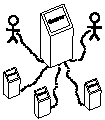
\includegraphics[scale=3]{serverrichpicture/server.pdf}
\caption{The server and the associated stations.}
\label{fig:ServerRichPicture}
\end{figure}

The dock that provide the locking and unlocking mechanism along with the bicycle detection ability have to communicate with the station. 
This is for example when they need to unlock a booked bicycle, the information needs to be propagated from the station to the individual dock containing the bicycle.
A sketch of how a station could look like when deployed can be seen in \figref{fig:StationRichPicture}.
The figure depicts a station and two docks connected to the station, which contains a bicycle each. 
On the display of the station, it can be seen that two bicycles are available for use.
\begin{figure}[h]
\centering

\includegraphics[scale=3]{stationrichpicture/station.pdf}
\caption{The station and the bicycles.}
\label{fig:StationRichPicture}
\end{figure}
	
	\chapter{Theory}
	Various theory needed as background information for the development of a solution is examined and discussed.\fxnote{her skal opremses hvad vi skriver om}
	\section{The Internet of Things}
This section introduces the Internet of Things (IoT), along with examples of how it is used. The section also introduces various hardware considerations to provide the context in which real-world applications for the IoT are developed.

The IoT is the concept describing the interconnection of uniquely identifiable objects in the problem domain.
The IoT also includes the virtual representation and the interfaces that allow for manipulation and information retrieval regarding objects \citep{misc:InternetOfThingsDefinition, misc:InternetOfThingsDefinition2, misc:InternetOfThingsDefinition3}.

Real usage of the IoT manifests as systems to provide some service, either by informing the user regarding things or allowing an intelligent system to manage those objects.
An example of this could be a so-called `smart home' that allows you to use a single device to manage the connected objects in your home, such as the lights or the oven in the kitchen \citep{misc:InternetOfThingsExamples}.
One society-wide use for it is the idea of a `Smart Grid', where the electricity usage is monitored and managed by an intelligent system that will e.g. redirect electricity if a cable has been cut somewhere in the system \citep{misc:smartGrid}.

There are already a lot of objects in the IoT, and by 2020 it is estimated that there will be upwards of around 26-30 billion things \citep{misc:IoTGrowth1,misc:IoTGrowth2}.
This will likely require a jump to the IPv6 protocol as the amount of IP addresses are severely limited by IPv4 \citep{misc:numberOfAddresses} given that the additions to IPv4, such as multiple devices sharing a single IP address, will at some point become insufficient.

One important aspect of the things connected to the IoT will be what technology they use to connect, here WiFi or mobile networking will not work well as they will likely interfere with one another.
The connectivity technology has to be low-power, cheap, and non-interfering.
One way to do that would be to directly connect objects to a server with a cable connecting to the internet, though that is not practical for objects that must be mobile.
RFID (Radio Frequency Identification) chips can provide relevant information to an outside observer about the object itself \citep{misc:rfid} with active research in making it low-cost and low-power \citep{misc:rfid2}.

The geographical location in the IoT is a good idea, especially for sensors where the location provides important context for the information of which something is accessing \citep{misc:locationMatters}.
For example if there is a station for bicycles in a bicycle sharing system that needs to provide information regarding the amount of bicycles at the station, it is important for the usage of the information that it also provides the actual location of the station, if that is not otherwise known.

In order to give more detail on IoT, aspecs about identification, communication, and software is given.

\subsection{Identification}

\subsection{Communication}

\subsection{Software}



In summary, the IoT has many challenges but at the same time also provides opportunities and benefits for society in general.
There are of course also criticism to it, primarily from a privacy point-of-view because it provides too much information.
	
	\afterpage{\thispagestyle{empty}}

	\bibliography{Bibliography}
	
	\label{lastpagewithoutappendix}

	\appendix
	%\input{Src/Appendix/File}
	
	\cleardoublepage
	\phantomsection
\end{document}
